% Compile with XeLaTeX from this directory; see README.md.
\documentclass[12pt,a4paper,oneside]{report}

\usepackage{fontspec}
\setmainfont{TeX Gyre Termes}
\setsansfont{TeX Gyre Heros}
\setmonofont{Latin Modern Mono}
\usepackage{polyglossia}
\setdefaultlanguage{vietnamese}
\setotherlanguage{english}

\usepackage[a4paper,top=2.5cm,bottom=2.5cm,left=3cm,right=2cm]{geometry}
\usepackage{graphicx}
\graphicspath{{../../figures/}}
\usepackage{booktabs,tabularx,longtable,array,multirow}
\usepackage{amsmath,amssymb}
\usepackage{siunitx}
\usepackage{float}
\usepackage{caption,subcaption}
\usepackage{enumitem}
\usepackage{xcolor}
\usepackage{fancyhdr}
\usepackage{hyperref}
\usepackage{url}
\usepackage{microtype}
\usepackage{setspace}
\usepackage{titlesec}

\definecolor{ptitblue}{HTML}{123B63}
\definecolor{softblue}{HTML}{EAF2F8}
\definecolor{warnred}{HTML}{8A1C1C}
\hypersetup{
  colorlinks=true,
  linkcolor=ptitblue,
  citecolor=ptitblue,
  urlcolor=ptitblue,
  pdftitle={Phân tích cảm xúc bình luận sản phẩm Điện Máy Xanh},
  pdfauthor={Nhóm 4 thành viên}
}
\setstretch{1.25}
\setlength{\parindent}{1.25cm}
\setlength{\parskip}{0.2em}
\setlist[itemize]{leftmargin=1.2cm,itemsep=0.2em}
\setlist[enumerate]{leftmargin=1.3cm,itemsep=0.2em}
\captionsetup{font=small,labelfont=bf}
\titleformat{\chapter}[display]
  {\normalfont\bfseries\color{ptitblue}\centering}
  {\Large CHƯƠNG \thechapter}{0.4em}{\Large}
\titlespacing*{\chapter}{0pt}{-12pt}{22pt}
\pagestyle{fancy}
\fancyhf{}
\fancyhead[L]{\small PTIT -- Phân tích và Khai phá Dữ liệu Văn bản}
\fancyhead[R]{\small Phân tích cảm xúc Điện Máy Xanh}
\fancyfoot[C]{\thepage}
\renewcommand{\headrulewidth}{0.4pt}
\newcolumntype{Y}{>{\raggedright\arraybackslash}X}
\newcommand{\Neg}{\textsc{Negative}}
\newcommand{\Neu}{\textsc{Neutral}}
\newcommand{\Pos}{\textsc{Positive}}
\newcommand{\PseudoLabel}{\textit{pseudo-label}}
\newcommand{\code}[1]{\texttt{\detokenize{#1}}}

\begin{document}
\begin{titlepage}
  \centering
  {\large HỌC VIỆN CÔNG NGHỆ BƯU CHÍNH VIỄN THÔNG\\[0.25em]
  KHOA / BỘ MÔN: [ĐIỀN TÊN KHOA/BỘ MÔN]}\\[2.2cm]
  {\large BÁO CÁO BÀI TẬP LỚN}\\[0.5em]
  {\large HỌC PHẦN: PHÂN TÍCH VÀ KHAI PHÁ DỮ LIỆU VĂN BẢN}\\[1.6cm]
  {\Huge\bfseries\color{ptitblue} PHÂN TÍCH CẢM XÚC BÌNH LUẬN SẢN PHẨM\\[0.4em]
  ĐIỆN MÁY XANH}\\[0.5cm]
  {\Large Vietnamese Product Review Sentiment Analysis}\\[1.8cm]
  \begin{tabular}{|c|p{5.0cm}|p{2.4cm}|p{4.0cm}|c|}\hline
    \textbf{STT} & \textbf{Họ và tên} & \textbf{Mã sinh viên} & \textbf{Phần việc chính} & \textbf{Tỷ lệ}\\\hline
    1 & [Thành viên 1] & [MSSV] & Thu thập dữ liệu, kiểm tra nhãn & [\%]\\\hline
    2 & [Thành viên 2] & [MSSV] & Tiền xử lý, đặc trưng, Naïve Bayes & [\%]\\\hline
    3 & [Thành viên 3] & [MSSV] & SVM, đánh giá và phân tích lỗi & [\%]\\\hline
    4 & [Thành viên 4] & [MSSV] & Transformer, notebook, tổng hợp báo cáo & [\%]\\\hline
  \end{tabular}\\[1.0cm]
  {\large Giảng viên hướng dẫn: [ĐIỀN HỌ TÊN GIẢNG VIÊN]}\\[0.6cm]
  {\large Hà Nội -- \today}
\end{titlepage}

\pagenumbering{roman}
\chapter*{Lời cam đoan}
Nhóm cam đoan nội dung báo cáo phản ánh đúng quy trình, mã nguồn và các kết quả đã thực hiện. Những biểu đồ tham khảo từ repository khác được phân biệt rõ với biểu đồ sinh trên dữ liệu Điện Máy Xanh. Các kết quả định lượng hiện tại được đánh giá trên nhãn tự động; nhóm không xem chúng là nhãn chuẩn do con người xác nhận.

\chapter*{Tóm tắt}
Báo cáo xây dựng pipeline phân loại cảm xúc ba lớp cho bình luận sản phẩm tiếng Việt trên Điện Máy Xanh. Dữ liệu được chuẩn hóa, tách từ và gán nhãn lai bằng rating kết hợp từ điển cảm xúc theo miền, quy tắc phủ định/cường độ và xử lý mâu thuẫn rating--văn bản. Sau lọc, tập dữ liệu gồm 9.516 bình luận duy nhất; 490 trường hợp mâu thuẫn được đánh dấu hoặc hiệu chỉnh. Nhóm so sánh Bag of Words (BoW), TF--IDF và Word2Vec với Naïve Bayes và Linear SVM. Trong lần thực nghiệm baseline đã lưu, Word2Vec + LinearSVC đạt Accuracy 0,828 và Macro-F1 0,695 trên tập test giữ lại. Lớp Neutral vẫn là lớp khó nhất, với F1 bằng 0,370. Mã nguồn hỗ trợ fine-tuning PhoBERT và XLM-RoBERTa Large, tuy nhiên chưa có kết quả fine-tuning Transformer được tạo trong lần chạy này.

\vspace{0.5em}
\noindent\textbf{Từ khóa:} phân tích cảm xúc, tiếng Việt, Điện Máy Xanh, TF--IDF, SVM, PhoBERT, XLM-RoBERTa.

\begin{center}
\colorbox{softblue}{\parbox{0.92\textwidth}{\textcolor{warnred}{\textbf{Cảnh báo về đánh giá:}} nhãn \code{label_target} và nhãn của \code{data/processed/test.csv} do quy tắc hybrid tự động tạo. Đây là đánh giá trên pseudo-label, không phải đánh giá trên tập gold được gán nhãn độc lập.}}
\end{center}

\tableofcontents
\listoffigures
\listoftables
\clearpage
\pagenumbering{arabic}

\chapter{Giới thiệu}

\section{Bối cảnh}
Đánh giá trực tuyến là nguồn dữ liệu quan trọng để người mua tham khảo và doanh nghiệp nhận biết vấn đề về chất lượng sản phẩm, giao hàng, lắp đặt và chăm sóc khách hàng. Số lượng bình luận lớn khiến việc đọc và tổng hợp thủ công tốn thời gian. Phân tích cảm xúc tự động có thể hỗ trợ sàng lọc phản hồi, theo dõi xu hướng và ưu tiên các phản ánh tiêu cực.

Tiếng Việt trong dữ liệu thương mại điện tử có nhiều đặc điểm gây khó khăn cho xử lý tự động: từ ghép nhiều âm tiết, viết tắt/teencode, lỗi chính tả, câu ngắn, cách nói khẩu ngữ, cấu trúc phủ định và câu vừa khen vừa chê. Một bình luận tích cực về giao hàng vẫn có thể phàn nàn về sản phẩm; do đó phân loại cảm xúc cần dựa trên ngữ cảnh thay vì chỉ dựa vào rating.

\section{Phát biểu bài toán}
Cho một bình luận sản phẩm tiếng Việt $x$, hệ thống dự đoán một trong ba lớp:
\begin{itemize}
  \item \textbf{Negative ($-1$):} phàn nàn, lỗi kỹ thuật, chất lượng thấp hoặc trải nghiệm dịch vụ kém;
  \item \textbf{Neutral ($0$):} thông tin trung lập, chưa đủ căn cứ, hoặc đánh giá pha trộn không nghiêng rõ;
  \item \textbf{Positive ($1$):} khen sản phẩm, dịch vụ, giao hàng hoặc trải nghiệm sử dụng.
\end{itemize}
Đây là phân loại cảm xúc cấp bình luận (document-level sentiment), chưa giải quyết đầy đủ cảm xúc đa khía cạnh trong cùng một câu.

\section{Mục tiêu và câu hỏi nghiên cứu}
Mục tiêu tổng quát là xây dựng pipeline có thể tái lập từ dữ liệu thô đến đánh giá, đồng thời phân tích vai trò của biểu diễn văn bản và mô hình. Các câu hỏi nghiên cứu gồm:
\begin{enumerate}
  \item BoW và TF--IDF cho kết quả khác nhau như thế nào với cùng bộ phân loại?
  \item Linear SVM có cải thiện Macro-F1 so với Naïve Bayes trên dữ liệu mất cân bằng không?
  \item Word2Vec mean pooling có giữ được tín hiệu cảm xúc so với các biểu diễn n-gram thưa không?
  \item Fine-tuning PhoBERT và XLM-RoBERTa Large có cải thiện hiệu năng các lớp thiểu số so với baseline cổ điển không?
  \item Các kiểu nhầm lẫn chính là gì, và mức độ nào có thể do nhiễu nhãn tự động?
\end{enumerate}

\section{Phạm vi và đóng góp}
Dự án sử dụng dữ liệu đánh giá sản phẩm công khai thuộc nhiều nhóm hàng của Điện Máy Xanh. Phạm vi triển khai gồm thu thập/chuyển đổi dữ liệu, chuẩn hóa tiếng Việt, tạo nhãn hybrid, trích chọn BoW/TF--IDF/Word2Vec, huấn luyện baseline/NB/SVM, xây dựng runner fine-tune PhoBERT/XLM-R, và tạo notebook LaTeX/report có thể tái lập.

Các đóng góp chính:
\begin{itemize}
  \item Tổ chức mã nguồn theo các mô-đun dữ liệu, đặc trưng, mô hình và đánh giá;
  \item Dùng nhãn kết hợp rating và từ điển cảm xúc để phát hiện trường hợp rating không khớp nội dung;
  \item So sánh các baseline trên cùng một split và báo cáo Macro-F1/per-class/confusion/CI;
  \item Nêu rõ giới hạn pseudo-label, thay vì diễn giải điểm số như chất lượng đã được xác thực bằng gold labels;
  \item Cung cấp mã cho Transformer hiện đại và quy trình lấy mẫu để đánh giá độc lập bằng người gán nhãn.
\end{itemize}

\section{Bố cục báo cáo}
Chương 2 giới thiệu cơ sở lý thuyết; Chương 3 mô tả dữ liệu, nhãn và pipeline; Chương 4 trình bày thiết kế thực nghiệm và kết quả hiện có; Chương 5 kết luận, giới hạn và hướng phát triển.

\chapter{Cơ sở lý thuyết}

\section{Phân tích cảm xúc}
Phân tích cảm xúc (sentiment analysis) là bài toán xác định thái độ hoặc cực tính cảm xúc được thể hiện trong văn bản. Trong nghiên cứu này, nhãn được quy về ba lớp. Lớp Neutral có ranh giới khó vì có thể biểu thị câu hỏi, mô tả thuần thông tin, trải nghiệm pha trộn, hoặc văn bản quá ngắn để xác định thái độ.

\section{Tiền xử lý tiếng Việt}
\subsection{Chuẩn hóa và tách từ}
Unicode NFC đưa các biểu diễn ký tự về dạng chuẩn; chuẩn hóa chữ hoa, URL, lặp ký tự và một số dạng teencode giúp giảm biến thể bề mặt. Tiếng Việt dùng khoảng trắng phân tách âm tiết chứ không luôn phân tách từ, do đó bộ tách từ nối các âm tiết của từ ghép thành token như \texttt{máy_giặt} và \texttt{bảo_hành}. PhoBERT được tiền huấn luyện trên dữ liệu tiếng Việt đã tách từ \cite{nguyen2020phobert}.

\subsection{Stopword, phủ định và liên từ chuyển ý}
Loại bỏ các hư từ phổ biến có thể giảm nhiễu trong BoW/TF--IDF, nhưng không được xóa từ phủ định như ``không'', ``chưa'', ``chẳng'' hoặc từ chỉ cường độ như ``rất'', ``hơi''. Các từ chuyển ý như ``nhưng'' thường báo hiệu mệnh đề sau mang kết luận quan trọng. Pipeline giữ các dấu hiệu này để tránh đảo nghĩa cảm xúc.

\section{Các phương pháp biểu diễn văn bản}
\subsection{Bag of Words}
BoW biểu diễn văn bản bằng số lần xuất hiện của từ hoặc n-gram. Phương pháp đơn giản, dễ giải thích và giữ lại cụm từ cục bộ như ``không tốt'', nhưng ma trận đặc trưng thưa và không mô hình hóa ngữ nghĩa xa.

\subsection{TF--IDF}
TF--IDF giảm trọng số các từ xuất hiện phổ biến trong nhiều văn bản và tăng vai trò tương đối của các từ mang tính phân biệt \cite{manning2008ir}. Dạng tổng quát:
\[
  \operatorname{tfidf}(t,d)=\operatorname{tf}(t,d)\times
  \log\frac{N}{1+\operatorname{df}(t)}.
\]
Thí nghiệm dùng unigram/bigram và sublinear term frequency.

\subsection{Word2Vec}
Word2Vec học vector từ dựa trên ngữ cảnh; dự án dùng Skip-gram và lấy trung bình vector từ trong bình luận (mean pooling) \cite{mik1989w2v}. Biểu diễn dense có thể gom các từ gần nghĩa nhưng phép lấy trung bình làm mất thứ tự từ và phạm vi phủ định.

\section{Các bộ phân loại}
\subsection{Naïve Bayes}
Naïve Bayes dự đoán lớp dựa trên định lý Bayes với giả định độc lập có điều kiện giữa các đặc trưng. MultinomialNB thích hợp với đặc trưng đếm hoặc TF--IDF không âm. GaussianNB được dùng cho vector Word2Vec liên tục.

\subsection{Support Vector Machine}
Linear SVM tìm siêu phẳng phân tách các lớp với biên lớn nhất; tham số $C$ điều khiển đánh đổi giữa độ rộng biên và lỗi huấn luyện. \texttt{class_weight=balanced} tăng mức phạt cho lớp ít mẫu \cite{cortes1995svm}.

\subsection{Transformer: PhoBERT và XLM-RoBERTa}
PhoBERT là mô hình ngôn ngữ tiền huấn luyện dành cho tiếng Việt, phù hợp làm encoder cho fine-tuning phân loại \cite{nguyen2020phobert}. XLM-RoBERTa được tiền huấn luyện đa ngôn ngữ quy mô lớn và là đối chứng để khảo sát năng lực chuyển giao xuyên ngôn ngữ \cite{conneau2020xlmr}. Trong mã nguồn, cả hai được nối với classification head và huấn luyện bằng weighted cross-entropy.

\textbf{Lưu ý:} checkpoint XLM-R Large và PhoBERT runner đã được tích hợp, nhưng báo cáo kết quả trong lần chạy này chưa bao gồm fine-tuning Transformer. Việc triển khai mã không đồng nghĩa với việc đã đo được hiệu năng của mô hình.

\section{Chỉ số đánh giá}
Với ba lớp, báo cáo Accuracy, Precision, Recall và F1 từng lớp; Macro-F1 là trung bình không trọng số giữa các lớp, còn Weighted-F1 cân theo support. Do lớp Positive chiếm đa số, Macro-F1 được chọn làm chỉ số chính để hạn chế việc Accuracy che khuất kết quả lớp hiếm.

Confusion matrix $C_{ij}$ cho biết số mẫu nhãn tham chiếu lớp $i$ được dự đoán thành lớp $j$. Chuẩn hóa theo hàng cho biết recall của mỗi lớp. Khoảng tin cậy Macro-F1 được ước lượng bằng bootstrap trên các mẫu test; khoảng này phản ánh bất định lấy mẫu có điều kiện trên bộ nhãn đang dùng, không hiệu chỉnh sai lệch của nhãn.

\chapter{Dữ liệu và phương pháp}

\section{Nguồn và mô tả dữ liệu}
Dữ liệu là các bình luận đánh giá sản phẩm công khai trên website Điện Máy Xanh, được lưu trữ tại \code{data/raw/}. Bảng \ref{tab:rating-raw} tổng hợp phân bố rating thô; các số liệu này mô tả dữ liệu crawl trước bước lọc và khử trùng lặp.

\begin{table}[H]
\centering
\caption{Phân bố rating trên 12.189 dòng thô}
\label{tab:rating-raw}
\begin{tabular}{lrr}
\toprule
Rating & Số mẫu & Tỷ lệ \\
\midrule
1 sao & 1.347 & 11,05\% \\
2 sao & 706 & 5,79\% \\
3 sao & 988 & 8,11\% \\
4 sao & 2.407 & 19,75\% \\
5 sao & 6.741 & 55,30\% \\
\midrule
Tổng & 12.189 & 100,00\% \\
\bottomrule
\end{tabular}
\end{table}

Các nhóm sản phẩm chính gồm tủ lạnh (3.366 dòng), nồi cơm điện (2.796), máy lạnh (2.030), máy giặt (1.725), máy lọc nước (1.724) và tivi (548). Phân bố rating lệch về 4--5 sao, vì vậy phân loại theo rating trực tiếp có thể tạo mất cân bằng lớp và không luôn phản ánh đúng nội dung văn bản.

\begin{figure}[H]
  \centering
  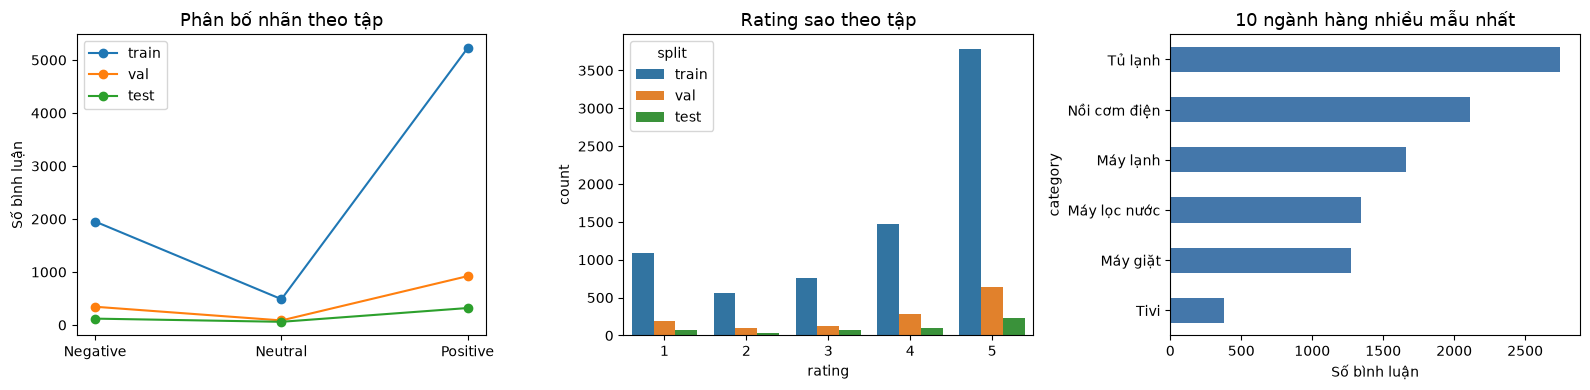
\includegraphics[width=\textwidth]{eda_data_overview.png}
  \caption{Tổng quan dữ liệu: phân bố nhãn theo split, rating theo split và số mẫu theo ngành hàng.}
  \label{fig:data-overview}
\end{figure}

\section{Làm sạch và tiền xử lý}
Quy trình xử lý được cài tại \code{src/data/preprocess.py} và gồm:
\begin{enumerate}
  \item bỏ nội dung rỗng, dạng lặp/ký tự vô nghĩa và bản ghi trùng theo cặp nội dung--rating;
  \item chuẩn hóa Unicode NFC, chữ thường, URL/HTML, teencode và một số lỗi chính tả/không dấu thường gặp;
  \item tách từ tiếng Việt bằng PyVi/Underthesea khi có sẵn, hoặc fallback miền thiết bị;
  \item tạo \code{text_segmented} cho PhoBERT (giữ cấu trúc và stopword) và \code{text_clean} cho ML cổ điển (lọc stopword nhưng bảo toàn phủ định/cảm xúc).
\end{enumerate}
Trong lần chạy hiện có, 49 dòng rác và 2.624 dòng trùng lặp bị loại; còn 9.516 review duy nhất hợp lệ.

\section{Gán nhãn hybrid và xử lý mâu thuẫn}
Nhãn sao ban đầu ánh xạ 1--2 sao thành Negative, 3 sao thành Neutral và 4--5 sao thành Positive. Bộ chấm lexicon miền thiết bị tại \code{src/data/auto_labeler.py} tính cực tính từ các từ tích cực/tiêu cực, điều chỉnh theo phủ định, cường độ và mệnh đề chuyển ý. Khi score văn bản mâu thuẫn mạnh với rating, quy tắc reconciliation có thể điều chỉnh nhãn đích. Quy trình lưu đồng thời \code{label_star}, \code{label_unsup}, \code{confidence}, \code{conflict_type} và \code{label_target} để có thể kiểm tra.

Trong 9.516 review hợp lệ, phân bố nhãn sao ban đầu là Negative 2.051 (21,55\%), Neutral 953 (10,01\%), Positive 6.512 (68,43\%). Sau reconciliation, nhãn đích là Negative 2.415 (25,38\%), Neutral 633 (6,65\%), Positive 6.468 (67,97\%). Có 490 trường hợp conflict được lưu để rà soát: 294 review ba sao có phàn nàn rõ; 79 review bốn--năm sao có nội dung tiêu cực mạnh; 67 review ba sao tích cực rõ; 41 review bốn sao pha trộn; và 9 review một--hai sao có nội dung tích cực.

\begin{figure}[H]
  \centering
  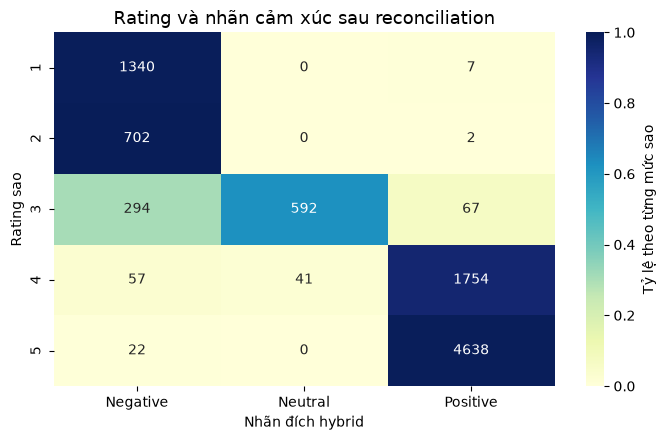
\includegraphics[width=0.78\textwidth]{rating_target_heatmap.png}
  \caption{Heatmap chéo giữa rating gốc và nhãn cảm xúc hybrid. Mỗi hàng được chuẩn hóa theo tỷ lệ rating; con số trong ô là số lượng mẫu.}
  \label{fig:rating-target}
\end{figure}

\begin{center}
\colorbox{softblue}{\parbox{0.92\textwidth}{\textbf{Giới hạn chất lượng nhãn.} Nhãn đích do quy tắc tự động tạo, chưa có đánh giá độc lập từ người gán. Vì vậy, các mô hình có thể học lại thiên lệch của lexicon/rating; chỉ số tại Chương 4 là mức đồng thuận với pseudo-label.}}
\end{center}

\section{Chia tập dữ liệu}
Dữ liệu được chia phân tầng theo \code{label_target} với seed 42. Các tập không có trùng lặp \code{review_id}. Split hiện tại là ngẫu nhiên theo review, không group theo mã sản phẩm; do đó cùng một sản phẩm có thể xuất hiện ở train và test.

\begin{table}[H]
\centering
\caption{Kích thước và phân bố nhãn của các split}
\label{tab:splits}
\begin{tabular}{lrrrr}
\toprule
Split & Tổng & Negative & Neutral & Positive \\
\midrule
Train & 7.664 & 1.951 & 487 & 5.226 \\
Validation & 1.352 & 344 & 86 & 922 \\
Held-out test & 500 & 120 & 60 & 320 \\
\bottomrule
\end{tabular}
\end{table}

Tập held-out được đặt tên \code{test.csv}, không dùng thuật ngữ ``gold test'' vì chưa gán thủ công. Vectorizer và Word2Vec chỉ fit trên train; validation phục vụ lựa chọn mô hình; test dùng đánh giá cuối.

\section{Thiết kế đặc trưng và mô hình}
\begin{table}[H]
\centering
\caption{Các nhánh thực nghiệm}
\label{tab:experiments}
\begin{tabularx}{\textwidth}{p{2.5cm}p{4.1cm}Y}
\toprule
Đặc trưng & Bộ phân loại & Mô tả cấu hình \\
\midrule
BoW & MultinomialNB, LinearSVC & CountVectorizer unigram/bigram, max 15.000 đặc trưng; NB $\alpha=1,0$, SVM $C=0,5$. \\
TF--IDF & MultinomialNB, LinearSVC & unigram/bigram, sublinear TF, max 15.000 đặc trưng; NB $\alpha=0,5$, SVM $C=1,0$. \\
Word2Vec & GaussianNB, LinearSVC & Skip-gram 100 chiều, window 5, min-count 2; vector câu mean pooling; SVM $C=1,0$. \\
Transformer & PhoBERT, XLM-R Large & Weighted cross-entropy, validation Macro-F1, early stopping; runner có sẵn nhưng chưa có kết quả fine-tune trong bảng hiện tại. \\
\bottomrule
\end{tabularx}
\end{table}
Naïve Bayes sử dụng hybrid resampling để giảm lệch lớp; SVM dùng trọng số lớp cân bằng. Majority baseline luôn dự đoán lớp có tần suất cao nhất.

\chapter{Thực nghiệm và kết quả}

\section{Thiết lập thực nghiệm}
Thí nghiệm baseline được chạy trên train = 7.664 mẫu, validation = 1.352 mẫu và held-out test = 500 mẫu. Tất cả mục tiêu đánh giá dùng cùng \code{label_target}. Baseline BoW/TF--IDF/Word2Vec sử dụng seed 42; Word2Vec Skip-gram chạy một worker để tăng khả năng tái lập. Macro-F1 được chọn làm chỉ số chính. Khoảng tin cậy percentile 95\% được ước lượng bằng 1.000 bootstrap resamples trên dự đoán test.

\section{Kết quả tổng hợp}
Bảng \ref{tab:leaderboard} cho thấy Word2Vec + LinearSVC có Macro-F1 test cao nhất trong các baseline đã chạy (0,6949), sát với BoW + MultinomialNB (0,6790). Majority baseline đạt Accuracy 0,640 nhưng Macro-F1 chỉ 0,2602 do không nhận diện hai lớp thiểu số. TF--IDF + LinearSVC có Accuracy cao nhất (0,830) nhưng Macro-F1 là 0,6626, thấp hơn Word2Vec + LinearSVC; điều này minh họa vì sao Accuracy không nên là tiêu chí duy nhất khi lớp bị mất cân bằng.

\begin{table}[H]
\centering
\caption{So sánh baseline trên held-out pseudo-labeled test}
\label{tab:leaderboard}
\small
\resizebox{\textwidth}{!}{%
\begin{tabular}{lrrrrrr}
\toprule
Mô hình & Accuracy & Macro-P & Macro-R & Macro-F1 & Weighted-F1 & Bootstrap CI 95\% (Macro-F1) \\
\midrule
Majority baseline & 0,640 & 0,2133 & 0,3333 & 0,2602 & 0,4995 & [0,2490; 0,2703] \\
BoW + MultinomialNB & 0,814 & 0,6742 & 0,6878 & 0,6790 & 0,8136 & [0,6305; 0,7270] \\
BoW + LinearSVC & 0,818 & 0,6906 & 0,6576 & 0,6632 & 0,8022 & [0,6144; 0,7100] \\
TF--IDF + MultinomialNB & 0,818 & 0,6578 & 0,6500 & 0,6378 & 0,7999 & [0,5936; 0,6881] \\
TF--IDF + LinearSVC & 0,830 & 0,6827 & 0,6688 & 0,6626 & 0,8130 & [0,6182; 0,7116] \\
Word2Vec + GaussianNB & 0,736 & 0,6060 & 0,6392 & 0,6119 & 0,7567 & [0,5703; 0,6593] \\
\textbf{Word2Vec + LinearSVC} & \textbf{0,828} & \textbf{0,6941} & \textbf{0,7038} & \textbf{0,6949} & \textbf{0,8246} & [0,6467; 0,7445] \\
\bottomrule
\end{tabular}}
\end{table}

\begin{figure}[H]
  \centering
  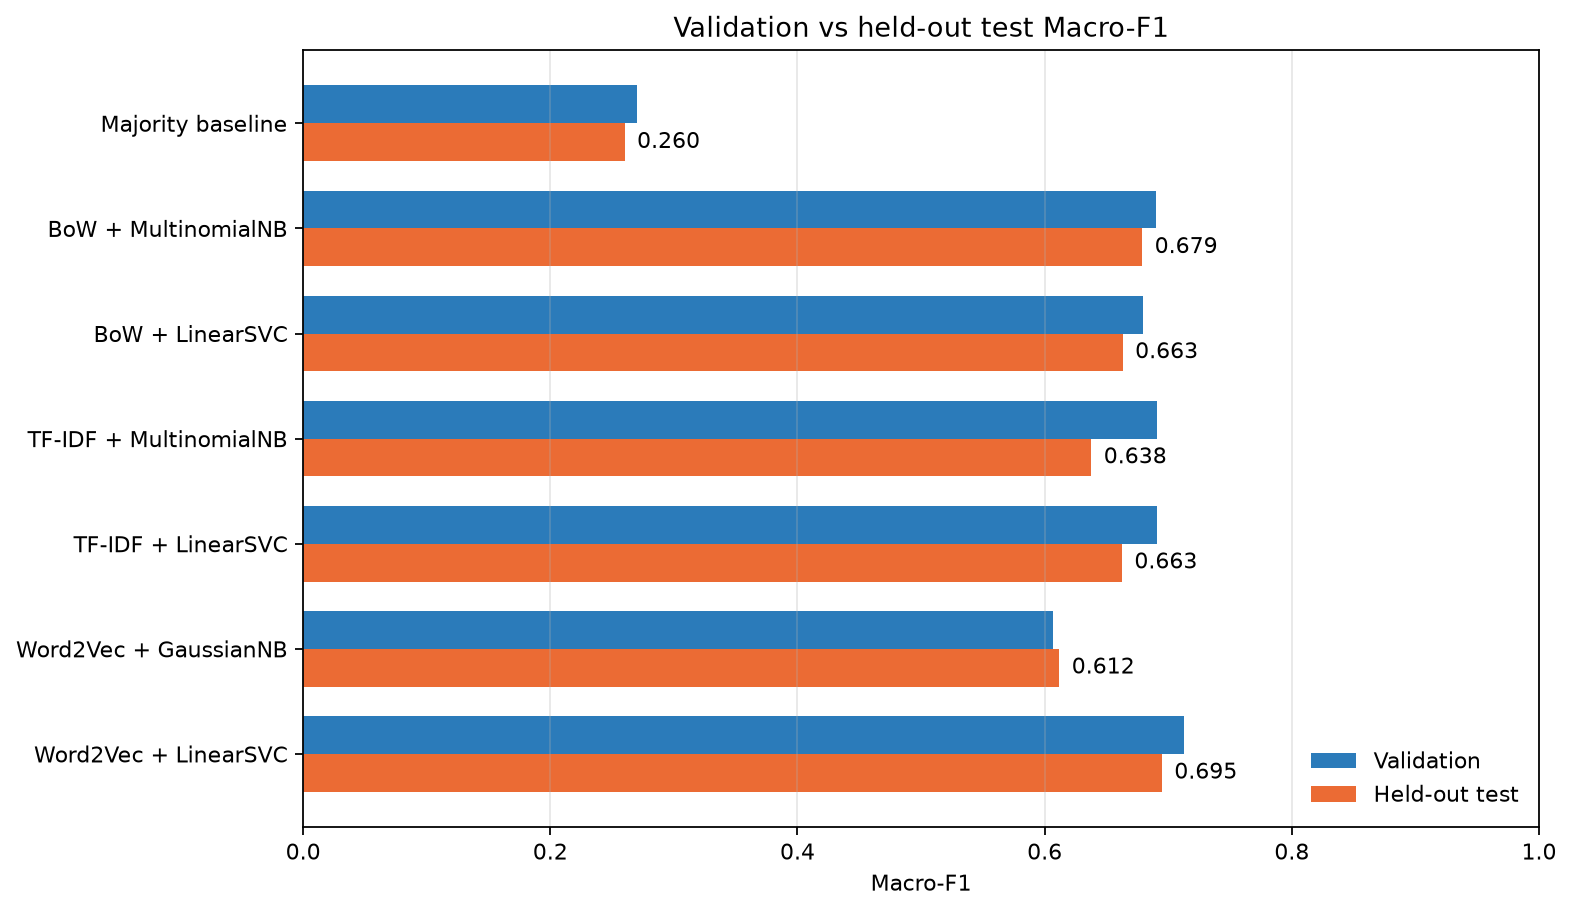
\includegraphics[width=0.92\textwidth]{macro_f1_val_test.png}
  \caption{Macro-F1 của các baseline trên validation và held-out test. Cả hai split sử dụng cùng nhãn đích hybrid.}
  \label{fig:macro-f1}
\end{figure}

\begin{figure}[H]
  \centering
  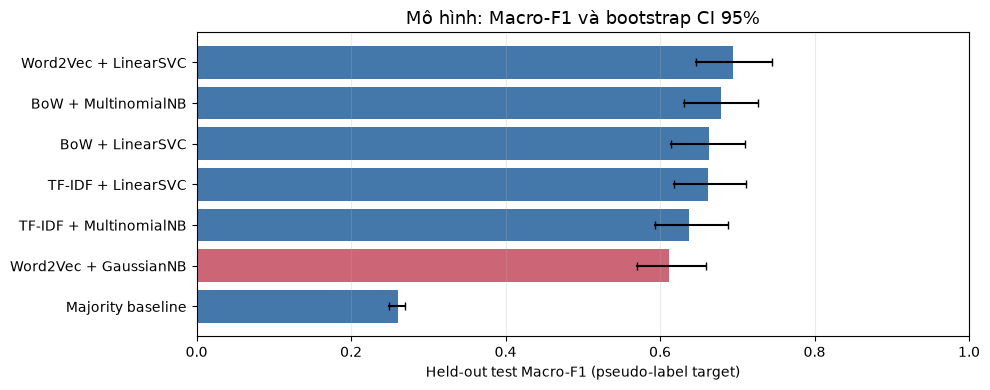
\includegraphics[width=0.90\textwidth]{macro_f1_test_ci.png}
  \caption{Macro-F1 trên held-out test kèm bootstrap CI 95\%. Các khoảng chồng lấp nên chênh lệch nhỏ cần được diễn giải thận trọng.}
  \label{fig:macro-f1-ci}
\end{figure}

Khoảng tin cậy giữa các mô hình có phần chồng lấp. Vì vậy, không kết luận chênh lệch nhỏ giữa các baseline là có ý nghĩa thống kê; kết quả cần được xác nhận bằng lặp seed/cross-validation và đặc biệt là nhãn được người gán độc lập.

\section{Phân tích theo lớp}
\begin{table}[H]
\centering
\caption{Chỉ số từng lớp của Word2Vec + LinearSVC}
\label{tab:per-class}
\begin{tabular}{lrrrr}
\toprule
Lớp & Precision & Recall & F1-score & Support \\
\midrule
Negative & 0,7241 & 0,8750 & 0,7925 & 120 \\
Neutral & 0,4167 & 0,3333 & 0,3704 & 60 \\
Positive & 0,9414 & 0,9031 & 0,9219 & 320 \\
\bottomrule
\end{tabular}
\end{table}

\begin{figure}[H]
  \centering
  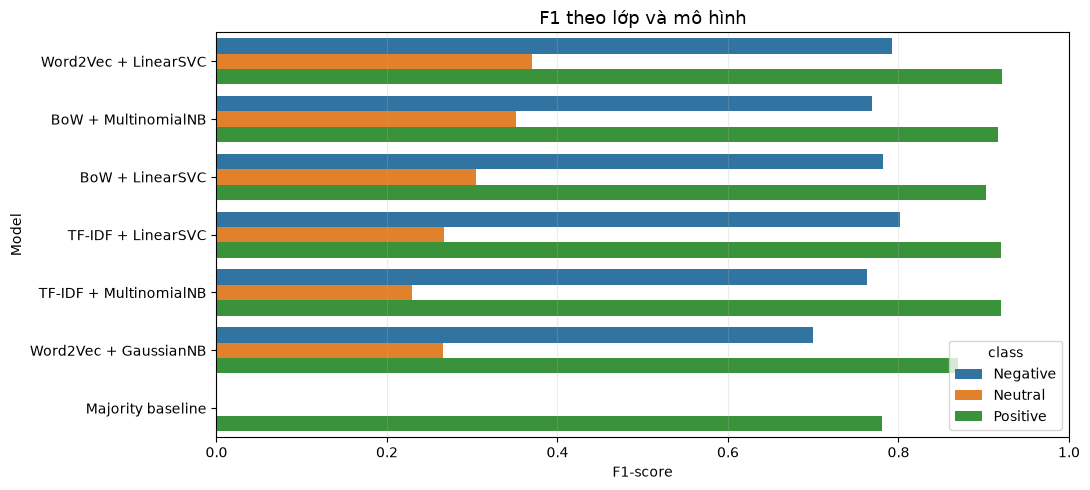
\includegraphics[width=0.93\textwidth]{per_class_f1_models.png}
  \caption{F1-score theo từng lớp và mô hình. Biểu đồ cho thấy hiệu năng lớp Neutral thường thấp hơn các lớp còn lại.}
  \label{fig:per-class-f1}
\end{figure}

Mô hình nhận diện tốt lớp Positive và Negative theo pseudo-label, nhưng lớp Neutral yếu hơn rõ rệt. Neutral chỉ có 60 mẫu trong test; nhiều bình luận trung tính ngắn hoặc pha trộn có thể bị đưa về cực tính lân cận. Với ứng dụng cảnh báo khiếu nại, recall Negative quan trọng để tránh bỏ sót phản ánh nghiêm trọng; trong kết quả hiện tại recall Negative là 0,8750. Tuy nhiên, các chỉ số này chịu ảnh hưởng trực tiếp của định nghĩa nhãn hybrid.

\section{Confusion matrix}
Với thứ tự nhãn tham chiếu và nhãn dự đoán là Negative, Neutral, Positive, ma trận số đếm của Word2Vec + LinearSVC là:
\[
\begin{bmatrix}
105 & 10 & 5 \\
27 & 20 & 13 \\
13 & 18 & 289
\end{bmatrix}.
\]
Có 86/500 dự đoán không khớp với pseudo-label. Trong 60 mẫu Neutral, 27 bị dự đoán thành Negative, 13 thành Positive và 20 được giữ đúng. Trong 320 mẫu Positive, 289 dự đoán đúng; 13 bị đưa về Negative và 18 về Neutral.

\begin{figure}[H]
  \centering
  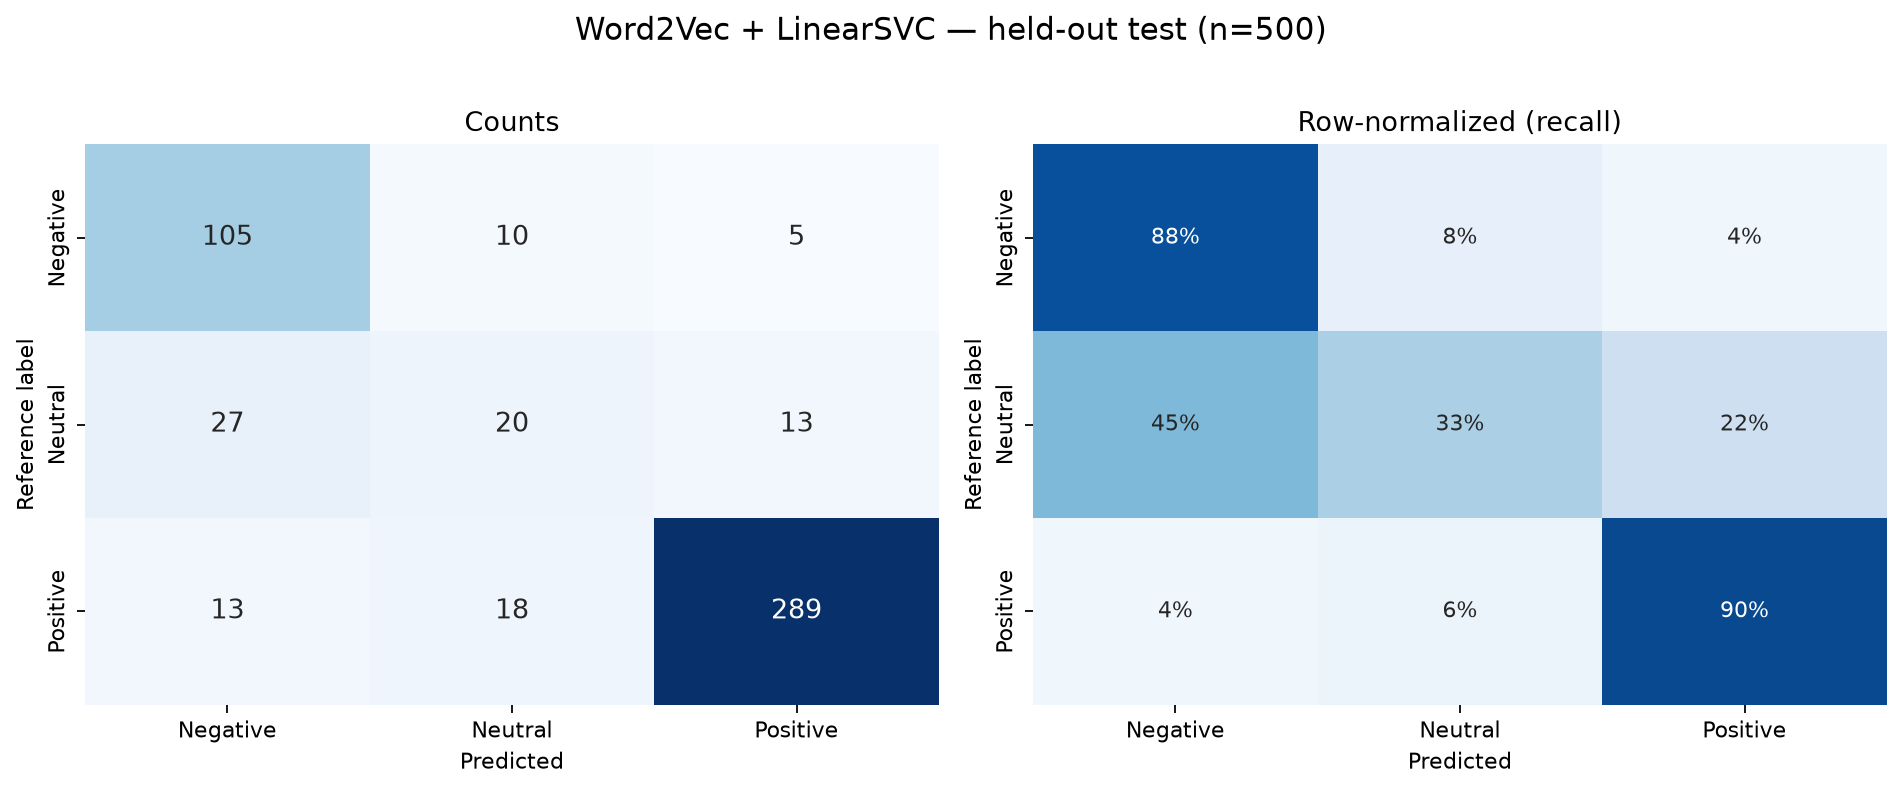
\includegraphics[width=0.95\textwidth]{cm_word2vec__linearsvc.png}
  \caption{Confusion matrix Word2Vec + LinearSVC trên held-out test (sinh từ dữ liệu Điện Máy Xanh trong repo).}
  \label{fig:cm-best}
\end{figure}

\section{Thảo luận và phân tích lỗi}
Các nhầm lẫn lớp Neutral phản ánh sự mơ hồ tự nhiên của nhiệm vụ: bình luận ``tạm ổn'', ``đẹp'', hoặc câu hỏi về sản phẩm có thể được gán khác nhau tùy ngữ cảnh và quy tắc gán nhãn. Một câu có cả lời khen dịch vụ lẫn phàn nàn về sản phẩm cũng khó rút về một nhãn cấp review. Bên cạnh đó, rating và lexicon vừa tạo target vừa quyết định trường hợp hiệu chỉnh, nên mô hình có thể học các tương quan của bộ quy tắc.

File dự đoán theo từng mẫu được lưu trong \code{outputs/predictions/word2vec__linearsvc.csv}; notebook cung cấp bảng xem lỗi theo lớp/ngành hàng để nhóm trích dẫn ví dụ sau khi rà soát. Các ví dụ nên được kiểm tra thủ công trước khi đưa nguyên văn vào bản báo cáo cuối.

\section{So sánh với mô hình Transformer}
Mã nguồn hiện hỗ trợ fine-tuning PhoBERT v2 trên văn bản đã tách từ và XLM-RoBERTa Large trên bình luận gốc, kèm weighted loss, validation Macro-F1 và early stopping. Tuy nhiên, chưa có artifact metrics Transformer trong lần chạy baseline này, vì vậy báo cáo không đưa điểm PhoBERT/XLM-R vào bảng và không khẳng định mô hình nào vượt trội. Sau khi chạy trên phần cứng phù hợp, cần bổ sung Macro-F1/per-class, confusion matrix, bootstrap interval, thời gian và cấu hình GPU; mọi mô hình phải được so sánh trên cùng split và cùng quy trình nhãn.

\section{Đe dọa tới giá trị đánh giá}
\begin{enumerate}
  \item \textbf{Pseudo-label bias:} test chưa gán độc lập; điểm số đo mức khớp với heuristic, không phải chân trị cảm xúc.
  \item \textbf{Split theo review:} cùng sản phẩm có thể xuất hiện ở train và test; kết quả có thể lạc quan nếu mô hình khai thác đặc điểm sản phẩm. Cần group split theo \code{product_code} cho đánh giá tổng quát hóa sản phẩm mới.
  \item \textbf{Mất cân bằng:} support Neutral nhỏ khiến ước lượng F1 lớp này biến động.
  \item \textbf{Lựa chọn mô hình:} các CI bootstrap chồng lấp; không nên tuyên bố ưu thế có ý nghĩa từ một lần split.
  \item \textbf{Tham số và tài nguyên:} thời gian huấn luyện cổ điển phụ thuộc môi trường; Transformer chưa được chạy nên chưa thể kết luận về trade-off chất lượng/chi phí.
\end{enumerate}

\chapter{Kết luận và hướng phát triển}

\section{Kết luận}
Nhóm đã xây dựng pipeline xử lý bình luận sản phẩm tiếng Việt từ dữ liệu thô đến huấn luyện và đánh giá các baseline. Pipeline gồm chuẩn hóa/word segmentation, lọc stopword bảo toàn phủ định, gán nhãn hybrid từ rating và lexicon, tạo split phân tầng, trích chọn BoW/TF--IDF/Word2Vec và huấn luyện Naïve Bayes/LinearSVC. Các artifact metrics, dự đoán và hình đánh giá được lưu để tái lập.

Trong thí nghiệm baseline đã chạy, Word2Vec + LinearSVC có Macro-F1 test cao nhất (0,6949) và Accuracy 0,828; Majority baseline có Macro-F1 0,2602. Kết quả theo lớp cho thấy Neutral còn khó (F1 0,3704), trong khi Positive và Negative có F1 cao hơn theo pseudo-label. Đây là phát hiện thực nghiệm ban đầu, không phải bằng chứng đã xác thực trên nhãn người gán.

\section{Hạn chế}
Hạn chế trọng yếu là toàn bộ nhãn train/validation/test hiện được sinh tự động. Reconciliation 490 trường hợp không đồng nghĩa đã xác nhận đúng cảm xúc, và đánh giá trên test cùng nguồn nhãn có thể khuyến khích vòng lặp tự củng cố. Ngoài ra, split chưa group theo sản phẩm, Neutral có support thấp, và các Transformer đã có mã nhưng chưa có kết quả thực nghiệm trong lần chạy báo cáo này.

\section{Hướng phát triển}
\begin{enumerate}
  \item Gán độc lập một tập con phân tầng bởi tối thiểu hai người, adjudicate bất đồng, tính Cohen's kappa và đánh giá lại mô hình trên nhãn đã kiểm định.
  \item Tạo benchmark group split theo sản phẩm, nhiều seed hoặc repeated cross-validation; giữ test độc lập khỏi mọi quyết định tuning.
  \item Fine-tune PhoBERT và XLM-R Large, báo cáo cùng protocol về Macro-F1, per-class scores, bootstrap interval và chi phí tính toán.
  \item Mở rộng lexicon theo ngành hàng, kiểm tra phủ định/phạm vi mệnh đề, xử lý câu đa khía cạnh và cân nhắc aspect-based sentiment.
  \item Đánh giá hiệu chỉnh xác suất, ngưỡng từ chối dự đoán và khả năng chuyển giao sang sản phẩm/thời điểm khác.
\end{enumerate}

\section{Biểu đồ nên có để đáp ứng yêu cầu bài tập}
Báo cáo phân cụm mẫu trình bày biểu đồ theo từng bước xử lý, biểu diễn kết quả thuật toán và dành phần riêng so sánh/diễn giải kết quả. Có thể kế thừa cách tổ chức đó, nhưng không dùng các biểu đồ Elbow, dendrogram, biểu đồ cụm RFM hay Silhouette của bài toán clustering cho phân loại cảm xúc. Với yêu cầu trong đề bài, nhóm nên ưu tiên các biểu đồ sentiment dưới đây:

\begin{table}[H]
\centering
\caption{Danh sách biểu đồ phù hợp cho hệ thống phân loại cảm xúc Điện Máy Xanh}
\label{tab:recommended-charts}
\small
\begin{tabularx}{\textwidth}{p{0.6cm}p{3.5cm}Yp{3.0cm}}
\toprule
Ưu tiên & Biểu đồ & Mục đích phân tích & Trạng thái trong repo \\
\midrule
Bắt buộc & Cột phân bố nhãn theo train/val/test và rating/category & Mô tả mất cân bằng, độ bao phủ ngành hàng và mức chênh giữa rating gốc với nhãn đích. Dùng số lượng hoặc tỷ lệ có ghi rõ mẫu số. & \code{eda_data_overview.png} \\
Bắt buộc & Heatmap rating $\times$ label target & Cho thấy reconciliation đã thay đổi nhãn ở đâu; dùng tỷ lệ theo hàng và ghi số lượng trong ô. & \code{rating_target_heatmap.png} \\
Bắt buộc & Bar chart Macro-F1 trên validation/test & So sánh biểu diễn (BoW, TF--IDF, Word2Vec) và thuật toán (NB, SVM); không chỉ dựa vào Accuracy. & \code{macro_f1_val_test.png} \\
Bắt buộc & Per-class Precision/Recall/F1, tốt nhất là grouped bars & Phân tích riêng Negative, Neutral và Positive, tránh để lớp đông chi phối kết luận tổng thể. & Bảng và hình \code{per_class_f1_models.png} \\
Bắt buộc & Confusion matrix số đếm + chuẩn hóa theo hàng & Xác định lớp/cặp nhầm lẫn; cần ít nhất mô hình tốt nhất và nên có top model NB/SVM. & Sinh cho từng baseline tại \code{figures/cm_*.png} \\
Nên có & Macro-F1 kèm bootstrap CI 95\% & Thể hiện bất định và tránh tuyên bố chênh lệch nhỏ là có ý nghĩa. & \code{macro_f1_test_ci.png} \\
Nên có & Error count theo ngành hàng và cặp nhầm lẫn & Phát hiện nhóm sản phẩm hoặc chủ đề dễ bị phân loại sai; bổ sung bảng ví dụ văn bản đã ẩn thông tin cá nhân. & Notebook có bảng; nên thêm stacked bar/heatmap nếu phân tích theo category. \\
Mở rộng & Precision--Recall curve one-vs-rest theo lớp & Hữu ích khi điều chỉnh threshold cho cảnh báo tiêu cực; lấy decision score/probability, không dùng nhãn cứng. & Chưa sinh mặc định; phù hợp khi lưu score của mô hình. \\
Mở rộng & Hiệu năng so với thời gian/VRAM; calibration/reliability plot & So sánh chất lượng và chi phí PhoBERT/XLM-R, đánh giá độ tin cậy confidence. & Chỉ thực hiện sau khi fine-tune Transformer. \\
\bottomrule
\end{tabularx}
\end{table}

\noindent\textbf{Quy tắc trình bày:} tất cả hình phải có tiêu đề/caption, tên trục, thứ tự lớp nhất quán (Negative, Neutral, Positive), nguồn dữ liệu và trạng thái nhãn (pseudo-label hay human-audited). Các hình trong \code{figures/reference/} không phải kết quả DMX và không được đưa vào phần kết quả.

\section*{Phân công nhóm bốn thành viên}
Bảng sau là khung để nhóm điền danh tính và tỷ lệ đóng góp thực tế; không điền tên hoặc tỷ lệ khi chưa có thông tin xác nhận.
\begin{table}[H]
\centering
\begin{tabularx}{\textwidth}{c p{3.2cm} p{2.3cm} Y c}
\toprule
STT & Họ và tên & MSSV & Phần việc & Tỷ lệ đóng góp \\
\midrule
1 & [Điền tên] & [Điền MSSV] & Thu thập dữ liệu, kiểm tra chất lượng và quy trình nhãn & [\%] \\
2 & [Điền tên] & [Điền MSSV] & Tiền xử lý, feature extraction, Naïve Bayes & [\%] \\
3 & [Điền tên] & [Điền MSSV] & SVM, đánh giá, confusion matrix và error analysis & [\%] \\
4 & [Điền tên] & [Điền MSSV] & PhoBERT/XLM-R, notebook, tích hợp và biên tập báo cáo & [\%] \\
\bottomrule
\end{tabularx}
\end{table}
\noindent Nhóm cần tự xác nhận tỷ lệ đóng góp sao cho tổng bằng 100\% và phản ánh đúng công việc đã thực hiện.


\begin{thebibliography}{99}
\bibitem{nguyen2020phobert}
D. Q. Nguyen and A. T. Nguyen, ``PhoBERT: Pre-trained language models for Vietnamese,'' in \textit{Findings of the Association for Computational Linguistics: EMNLP 2020}, pp. 1037--1042, 2020. doi: 10.18653/v1/2020.findings-emnlp.92.

\bibitem{conneau2020xlmr}
A. Conneau et al., ``Unsupervised Cross-lingual Representation Learning at Scale,'' in \textit{Proceedings of ACL 2020}, pp. 8440--8451, 2020. doi: 10.18653/v1/2020.acl-main.747.

\bibitem{cortes1995svm}
C. Cortes and V. Vapnik, ``Support-vector networks,'' \textit{Machine Learning}, vol. 20, pp. 273--297, 1995. doi: 10.1007/BF00994018.

\bibitem{manning2008ir}
C. D. Manning, P. Raghavan, and H. Schütze, \textit{Introduction to Information Retrieval}. Cambridge University Press, 2008.

\bibitem{mik1989w2v}
T. Mikolov, K. Chen, G. Corrado, and J. Dean, ``Efficient Estimation of Word Representations in Vector Space,'' arXiv:1301.3781, 2013.

\bibitem{sklearn}
F. Pedregosa et al., ``Scikit-learn: Machine Learning in Python,'' \textit{Journal of Machine Learning Research}, vol. 12, pp. 2825--2830, 2011.

\bibitem{dmx}
Điện Máy Xanh, ``Đánh giá sản phẩm,'' dữ liệu đánh giá công khai được thu thập phục vụ bài tập lớn, 2025. Truy cập: \url{https://www.dienmayxanh.com/}.

\bibitem{lazada-template}
Học viện Công nghệ Bưu chính Viễn thông, \textit{Bài Tập Lớn I -- Lazada.pdf}, tài liệu mẫu báo cáo môn học do nhóm sử dụng tham khảo bố cục.

\bibitem{clustering-template}
Học viện Công nghệ Bưu chính Viễn thông, \textit{Bài tập lớn 1 -- Clustering.pdf}, báo cáo mẫu do người dùng cung cấp để tham khảo cách chia chương, trình bày quy trình, diễn giải kết quả và tổ chức đóng góp thành viên. Chủ đề và các biểu đồ clustering không được áp dụng như kết quả sentiment.
\end{thebibliography}

\appendix
\chapter{Tái lập thực nghiệm}
Mã nguồn, cấu hình và notebook được quản lý trong repository \code{dmx-nlp-sentiment}. Các lệnh chạy chính:
\begin{verbatim}
python auto_label_review.py
python scripts/train_classical.py --bootstrap 1000
python scripts/train_transformer.py --model-name vinai/phobert-base-v2
python scripts/train_transformer.py --model-name FacebookAI/xlm-roberta-large \
  --batch-size 2 --gradient-accumulation-steps 8
jupyter lab notebooks/01_sentiment_analysis_report.ipynb
\end{verbatim}
Checkpoint Transformers cần tải từ Hugging Face và có thể cần GPU. Kết quả báo cáo trong bản hiện tại bao gồm baseline cổ điển; không đưa số liệu Transformer nếu chưa chạy script tương ứng.

\chapter{Lưu ý về hình tham khảo}
Các ảnh trong \code{figures/reference/} là biểu đồ tham khảo từ repository khác cùng chủ đề, không phải kết quả của Điện Máy Xanh. Báo cáo này chỉ sử dụng các hình mới được sinh trong thư mục \code{figures/} ở mức gốc, ví dụ \code{macro_f1_val_test.png} và \code{cm_word2vec__linearsvc.png}.

\end{document}
